\documentclass[utf8]{jetp}

\usepackage{amsmath}
\usepackage{amssymb}

\usepackage{soul,color}
\usepackage{textcomp}

\usepackage{lineno}
\modulolinenumbers[1]
\linenumbers

\newcommand{\tr}[1]{\mathrm{Tr} \left\{ #1 \right\}}
\newcommand{\sx}{I_\mathrm{x}}
\newcommand{\sy}{I_\mathrm{y}}
\newcommand{\sz}{I_\mathrm{z}}
\newcommand{\hdz}{H_\mathrm{dz}}


\bibliographystyle{unsrt}

%%%%%%%%%%%%%%%%%%%%%%%

\begin{document}

\title{Многоспиновая запутанность в многоквантовом~ЯМР~с дипольном упорядоченным начальным состоянием}

\author{И.~Д.}{Лазарев}
\email{ilia.lazarev@icp.ac.ru}
\affiliation{Институт проблем химической физики РАН, \\ Черноголовка, Московская область, Россия 142432}
\affiliation{Факультет фундаментальной физико-химической инженерии, \\ МГУ GSP-1, Москва, Россия 119991}

\author{Э.~Б.}{Фельдман}
\affiliation{Институт проблем химической физики РАН, \\ Черноголовка, Московская область, Россия 142432}

\abstract{
Многоквантовый (МК)~ЯМР~с~дипольном упорядоченным начальным состоянием открывает новые возможности для изучения многоспиновой запутанности.
В~данной статье исследуется многоспиновая запутанность в~газе спин-несущих молекул (атомов) в нанопоре
в~условиях~ЯМР~с дипольном упорядоченным начальным состоянием.
Для~оценки количества запутанных спинов используется второй момент распределения МК~интенсивностей~ЯМР~когерентностей,
который определяет нижнюю границу квантовой информации Фишера.
Многоспиновая запутанность исследуется при различных температурах и различном количестве спинов.
}

% \begin{keyword}
% многоквантовый (МК)~ЯМР~\sep
% квантовые корреляции \sep
% квантовая информация Фишера \sep
% запутанность, нанопора \sep
% МК~когерентностъ~ЯМР \sep
% второй момент, температура \sep
% дипольном упорядоченное состояние \sep
% двухимпульсная последовательность Брукерта-Джинера
% \end{keyword}

%\linenumbers

\maketitle

\section{Введение}
\label{sec:1}

Запутанность~\cite{Nielsen_2009} является важной концепцией квантовой механики.
В частности, она ответственна за преимущество квантовых компьютеров перед их классическими аналогами.
Недавно продемонстрированное квантовое превосходство~\cite{Arute2019} на программируемом сверхпроводящем процессоре также связано с понятием запутанности, которое отсутствует в классической физике.
Среди многочисленных методов исследования запутанности мы сосредоточились на многоквантовом~(МК)~ЯМР в~твердых телах~\cite{Baum_1985},
который широко используется для изучения запутанности в бинарных системах~\cite{Furman_2008, Furman_2009, Fel_dman_2008, Fel_dman_2012}.

Оказалось также, что МК~спектроскопия~ЯМР~\cite{Baum_1985} позволяет извлекать информацию о многоспиновой запутанности~\cite{G_rttner_2018} с~помощью квантовой информации Фишера~\cite{T_th_2014, Pezz__2018},
являющейся ключевой концепцией в квантовой теории информации.
Квантовая информация Фишера описывает скорость изменения квантовых состояний,
определяемых матрицей плотности, при изменении наблюдаемой,
которая определяет МК когерентности ЯМР в~МК~спектроскопии~ЯМР~~\cite{Baum_1985}.
В МК спектроскопии ЯМР эта наблюдаемая определяется оператором полной проекции углового спинового момента на направление сильного внешнего магнитного поля.
Используя квантовую информацию Фишера~\cite{Liu_2014} для анализа МК~спектра~ЯМР,
можно получить важную информацию о многоспиновой запутанности,
поскольку существует связь между вторым моментом спектра~\cite{Khitrin_1997} и квантовой информацией Фишера~\cite{G_rttner_2018,Doronin_2019}.
Кроме того второй момент МК~спектра~ЯМР~определяет нижнюю границу квантовой информации Фишера~\cite{G_rttner_2018}.
Это означает, что МК~спектроскопия~ЯМР является эффективным методом решения квантовых информационных задач.

Многоспиновая запутанность была исследована~\cite{Doronin_2019} для несферической нанопоры,
заполненной газом  спин-несущих молекул в сильном внешнем магнитном поле~\cite{Baugh_2001,Doronin_2009}.
Термодинамически равновесное начальное состояние системы определялось односпиновым зеемановским взаимодействием с внешним магнитным полем~\cite{Doronin_2007a}.
Однако  многоспиновую запутанность можно  исследовать,
когда та же самая система первоначально подготовлена в дипольном упорядоченном состоянии~\cite{Goldman_1970},
используя либо метод адиабатического размагничивания во вращающейся системе координат (ВСК)~\cite{Goldman_1970, Slichter_1961},
либо двухимпульную последовательность Брокаерта-Джинера~\cite{Goldman_1970, Jeener_1967}.
МК~динамика~ЯМР~с таким начальным состоянием моделировалась как для небольших спиновых систем~\cite{Doronin_2007a, Doronin_2007b},
так и в системе, состоящей из 200-600 спин-несущих молекул (атомов), заполняющих нанопору~\cite{Doronin_2011}.
Однако подходы, разработанные для этих исследований, ограничены случаем высоких температур и не могут применяться  для изучения многоспиновой запутанности.

В настоящей статье мы рассматриваем промежуточный температурный случай с низкой зеемановской и высокой дипольной температурами.
Магнитное упорядочение~\cite{Abragam_1982} выходит за рамки данной статьи.
Заметим, что двухимпульсный эксперимент Брокаерта-Джинира~\cite{Jeener_1967} был разработан для высокотемпературного случая.
Мы теоретически  показываем, что этот эксперимент~\cite{Jeener_1967} также может выполняться и для промежуточного температурного случая, рассматриваемого в настоящей статье.
Было показано~\cite{Doronin_2011}, что в МК~эксперименте~ЯМР~с дипольном упорядоченным начальным состоянием МК~когерентности~ЯМР~возникают быстрее,
чем в МК~эксперименте~ЯМР~с начальным термодинамическим равновесным состоянием в сильном внешнем магнитном поле.
Данное обстоятельство является важным для исследования многоспиновой запутанности, поскольку при этом используется  второй момент распределения МК~когерентностей~ЯМР~.
Указанное обстоятельство также важно для исследования распространения многоспиновых корреляций~\cite{Baugh_2001,Baum_1986,S_nchez_2014,Munowitz_1987} и локализации~\cite{Alvarez_2015,Wei_2018}.
При этом важную роль играют неупорядоченные по времени корреляции (out-of-time ordered correlations), которые связаны с распределением МК~когерентностей~ЯМР.

В данной статье исследуется многоспиновая запутанность с использованием МК  спектра~ЯМР~спин-несущих атомов (молекул) в нанопоре, когда система приготовлена в дипольном упорядоченном состоянии.
В разделе~\ref{sec:2} описана разработанная теория МК~динамики~ЯМР~при низкой зеемановской температуре и высокой дипольной температуре.
Аналитическое решение для МК~динамики~ЯМР трехспиновой системы, полученное при таких же температурах,  описано в разделе~\ref{sec:3}.
Второй момент МК~спектра~ЯМР~в качестве меры многоспиновой запутанности рассматривается в разделе~\ref{sec:4}.
В разделе~\ref{sec:5} исследуется зависимость многоспиновой запутанности от дипольной температуры и числа спинов в системе.
Краткое изложение полученных результатов приведено в разделе~\ref{sec:6}.
В Приложении показано, что двухимпульсная последовательность Брокаерта-Джинера может быть использована в случае, когда зеемановская температура низкая, а дипольная - высокая.



\section{Теория МК~динамики~ЯМР~в нанопоре при низкой зеемановской  и высокой дипольной температурах}
\label{sec:2}

МК~динамика~ЯМР~в нанопоре определяется гамильтонианом~\cite{Doronin_2019,Doronin_2009}
%
\begin{equation}
  \label{eq:1}
  H_{\mathrm{MQ}} = - \dfrac{D}{4} \left[
    \left(I^{+}\right)^{2}
    + \left(I^{-}\right)^{2}
  \right] ,
\end{equation}
%
где
%
\begin{equation}
  \label{eq:2}
  I^{\pm} = \sum\limits_{j=1}^{N} I_{j}^{\pm},
\end{equation}
%
где $N$ - число спинов в нанопоре, $I^{\pm}_{j}$ - повышающий или понижающий операторы спина $j$, $D$ - константа диполь-дипольного взаимодействия (ДДВ),
усредненная по быстрой молекулярной диффузии спин-несущих атомов (молекул) в нанопоре.
Подчеркнем, что константа ДДВ $D$ одинакова для всех пар взаимодействующих спинов в нанопоре~\cite{Doronin_2019,Doronin_2009}.
Матрица плотности $\rho(\tau)$ на подготовительном периоде МК~эксперимента~ЯМР~\cite{Baum_1985} может быть получена из эволюционного уравнения Лиувилля~\cite{Goldman_1970,Abragam_1982}
%
\begin{equation}
  \label{eq:3}
  i\dfrac{\mathrm{d}\rho(\tau)}{\mathrm{d}\tau} = \left[
  H_\mathrm{MQ},\rho(\tau)
  \right]
\end{equation}
%
с начальной термодинамической равновесной матрицей плотности
%
\begin{equation}
  \label{eq:4}
    \rho(0) = \rho_\mathrm{eq} = \dfrac{1}{Z}
    e^{
      \frac{\hslash \omega}{k} \alpha_\mathrm{z} I_\mathrm{z}
      + \frac{\hslash }{k} \beta_\mathrm{d} H_\mathrm{dz}
    },
\end{equation}
%
где
$Z = \mathrm{Tr} \left\{ e^{\frac{\hslash \omega}{k} \alpha_\mathrm{z} I_\mathrm{z} + \frac{\hslash }{k} \beta_\mathrm{d} H_\mathrm{dz}} \right\}$ - статистическая сумма,
$\hslash$ и $k$ - константы Планка и Больцмана,
$\omega_{0}$ - частота Лармора ,
$I_\mathrm{z}$ -  оператор проекции полного углового спинового момента  на ось~$z$,
который направлен вдоль сильного внешнего магнитного поля,
$H_\mathrm{dz}$ - секулярная часть гамильтониана ДДВ в сильном внешнем магнитном поле
и $\alpha_\mathrm{z}$, $\beta_\mathrm{d}$ - обратные зеемановская и дипольная температуры.
Мы рассмотрим случай, когда зеемановская температура  является низкой $({\frac{\hslash \omega}{k} \alpha_\mathrm{z}}\gg 1)$,
а дипольная - высокой $\left( \frac{\hslash{D}}{k}\beta_\mathrm{d} \ll 1\right)$.
Мы предполагаем, что $\omega_{0} = 2\pi \cdot 500 \cdot 10^{6}$~s$^{-1}$ и $D = 2\pi \cdot 10^{4}$~s$^{-1}$.
В приложении мы доказываем, что двухимпульсная последовательность Брокаерта-Джинера~\cite{Goldman_1970,Jeener_1967} позволяет получить дипольном упорядоченное состояние даже при низкой зеемановской температуре.
Другим методом создания  дипольном упорядоченного состояния системы является адиабатическое размагничивание~\cite{Goldman_1970,Slichter_1961}.
Используя эти методы, мы можем получить систему в состоянии термодинамического равновесия с матрицей плотности
%
\begin{equation}
  \label{eq:5}
  \rho_i = \frac{1}{Z_i} e^\frac{\hslash\beta_\mathrm{d} \hdz}{k}
  \approx \frac{1}{Z_i}(1 + \frac{\hslash\beta_\mathrm{d}}{k} H_\mathrm{dz}),
\end{equation}
%
где статистическая сумма
%
\begin{equation}
  \label{eq:6}
	Z_i = \mathrm{Tr} \left\{ e^\frac{\hslash\beta_\mathrm{d} \hdz}{k} \right\} \approx 2^{N}.
\end{equation}
%
МК~динамика~ЯМР~в нанопоре будет исследована на основе уравнения~(\ref{eq:3}) с начальным состоянием~(\ref{eq:5}).
Также важно отметить, что гамильтониан $H_{dz}$ частично усредняется быстрой молекулярной диффузией в нанопоре, а усредненный гамильтониан можно записать как \cite{Fel_dman_2004,Doronin_2011}
%
\begin{equation}
  \label{eq:7}
  H_\mathrm{dz} = \dfrac{D}{2} (3 I^{2}_{z} - I^{2}) , % ?
\end{equation}
%
где $I^{2}$ - квадрат углового спинового  момента.

Пусть $G(\tau,\phi)$ описывает усредненный по равновесной матрице плотности сигнал после периодов подготовки, эволюции и смешивания в МК~эксперименте~ЯМР~\cite{Baum_1985}.
$G(\tau,\phi)$ может записать как~\cite{Doronin_2019}
%
\begin{equation}
  \begin{split}
    \label{eq:8}
    G(\tau,\phi)
    & = \mathrm{Tr}\left\{
      e^{i H_\mathrm{MQ} \tau} e^{i\phi I_\mathrm{z}} e^{-i H_\mathrm{MQ}\tau}
      \rho_i
      e^{i H_\mathrm{MQ} \tau} e^{-i \phi I_\mathrm{z}} e^{-i \phi H_\mathrm{MQ} \tau}
      \rho_i
    \right\} \\
    & = \mathrm{Tr} \left\{
    e^{i \phi I_\mathrm{z}}
    \rho(\tau)
    e^{-i \phi I_\mathrm{z}}
    \rho(\tau)
    \right\},
  \end{split}
\end{equation}
%
где
%
\begin{equation}
  \label{eq:9}
  \rho(\tau)
  = e^{-i H_\mathrm{MQ} \tau }
  \rho_i
  e^{i H_\mathrm{MQ} \tau}
\end{equation}
%
является решением уравнения~(\ref{eq:3}) при начальном условии~(\ref{eq:5}).
Матрица плотности $\rho(\tau)$ раскладывается в ряд
%
\begin{equation}
  \label{eq:10}
  \rho(\tau) = \sum\limits_n \rho_n(\tau),
\end{equation}
%
где $\rho_{n}(\tau)$ - вклад в $\rho(\tau)$ от МК~когерентности $n$-го порядка~\cite{Fel_dman_1996}.
Тогда  функцию $G(\tau,\phi)$ в уравнении~(\ref{eq:8}) можно переписать как
%
\begin{equation}
  \label{eq:11}
  G(\tau,\phi)
  = \sum\limits_n e^{i n \phi} \mathrm{Tr} \left\{
    \rho_{n}(\tau) \rho_{-n}(\tau)
  \right\},
\end{equation}
%
где мы учитываем, что
%
\begin{equation}
  \label{eq:12}
  \left[ I_{\mathrm{z}},\rho_n(\tau) \right] = n \rho_n(\tau)
\end{equation}
%
Для дальнейших расчетов необходимо ввести нормированные интенсивности $J_{n}(\tau)$ $(n=0, \pm 2, \pm 4, \cdots)$ МК~когерентностей~ЯМР
%
\begin{equation}
  \label{eq:13}
  J_{n}(\tau) = \dfrac{\mathrm{Tr} \left\{
  \rho_{n}(\tau) \rho_{-n}(\tau)
  \right\}}
  {\mathrm{Tr} \left\{\rho^2_{i} \right\}}
\end{equation}
%
Используя уравнения~(\ref{eq:9}),~(\ref{eq:10}), можно проверить, что
%
\begin{multline}
  \label{eq:14}
  \sum\limits_{n} J_{n}(\tau)
  = \dfrac{
    \mathrm{Tr} \left\{
      \sum_{n} \rho_{n}(\tau) \rho_{-n}(\tau)
    \right\}}
  {\mathrm{Tr} \left\{ \rho^2_{i} \right\}}
  = \dfrac{
    \mathrm{Tr} \left\{
      \sum_{\mathrm{m,n}} \rho_n(\tau)\rho_m(\tau)
  \right\}}
  {\mathrm{Tr} \left\{\rho^2_{i}\right\}}
  \\
  = \dfrac{
    \mathrm{Tr}\left\{\rho^2(\tau)\right\}
  }
  {
    \mathrm{Tr}\left\{\rho^2_{i}(\tau)\right\}
  }
  = \dfrac{
    \mathrm{Tr} \left\{
      e^{-i H_\mathrm{MQ} \tau}
      \rho^{2}_{i}
      e^{i H_\mathrm{MQ} \tau}
    \right\}
  }
  {
    \mathrm{Tr} \left\{ \rho_{i}^{2} \right\}
  }
  = 1
\end{multline}
%
Из уравнения~(\ref{eq:14}) можно сделать вывод, что сумма МК~когерентностей~ЯМР~сохраняется на подготовительном периоде МК~эксперимента~ЯМР~\cite{Baum_1985}.

Базис, состоящий из собственных состояний оператора $I_\mathrm{z}$ (называемый мультипликативным базисом), широко используется для численных расчетов МК~динамики~ЯМР~\cite{Zhang_2009}.
В связи с быстрым расширением гильбертова пространства с ростом числа спинов такие вычисления возможны только для систем с небольшим числом спинов.
Такой подход не подходит для исследований многоспиновой запутанности.
Поскольку гамильтониан $H_{MQ}$ уравнения~(\ref{eq:1}) коммутирует с квадратом полного углового момента спина $\hat I^2$,
можно использовать базис, состоящий из общих собственных состояний $\hat I^2$ и $I_\mathrm{z}$ для изучения МК~динамики~ЯМР, как это было сделано в статьях~\cite{Doronin_2009,Doronin_2011,Doronin_2019}.
В этом базисе гамильтониан $H_{MQ}$ и исходная матрица плотности~(\ref{eq:5}) (см. также~(\ref{eq:7})) состоят из блоков, соответствующих различным значениям углового момента спина~\cite{Doronin_2009}.
Тогда исследование МК~динамики~ЯМР~может быть сведено к решению ряда задач меньших размеров.

Поскольку гамильтониан $H_{MQ}$ уравнения~(\ref{eq:1}) коммутирует с оператором $e^{i\pi I_\mathrm{z}}$, то $2^N \times 2^N$ матрица гамильтониана сводится к двум блокам $2^{N-1} \times 2^{N-1}$~\cite{Doronin_2009}.
Для нечетных $N$ оба блока вносят одинаковый вклад в МК~когерентности~ЯМР~, и можно решить проблему, используя только один блок $2^{N-1} \times 2^{N-1}$, и удвоить полученные интенсивности.
В наших расчетах мы берем только нечетные числа спинов.
Используя этот метод, можно исследовать МК~динамику~ЯМР~в системах, состоящих и сотен спинов.

\section{Аналитическое решение для МК~динамики~ЯМР~трехспиновой системы в нанопоре в дипольном упорядоченном состоянии}
\label{sec:3}

\begin{figure}
  \centering
 	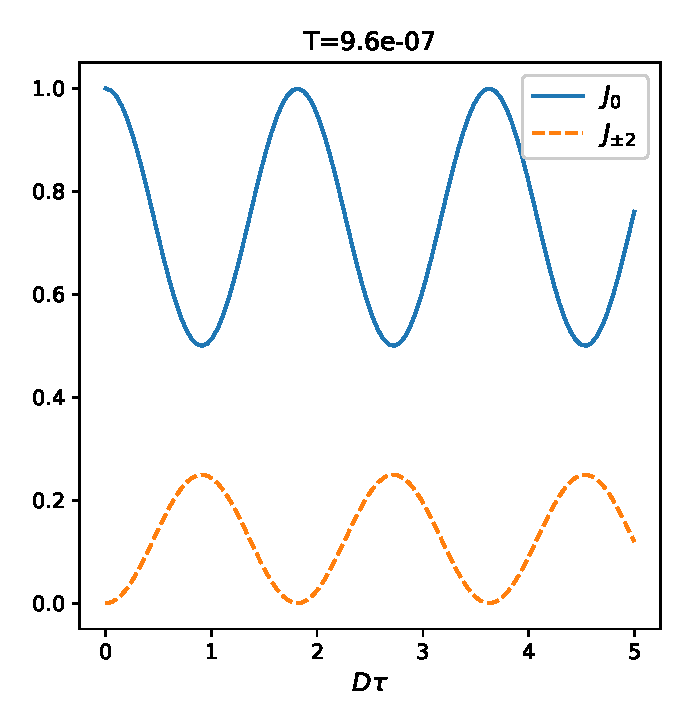
\includegraphics[width=0.5\linewidth]{coherences_n3_beta5.eps}
	\caption{
	  Интенсивности МК~когерентностей~ЯМР~$J_{n}$ ($n=0, 2$) в нанопоре с $N=3$.
	}
	\label{fig:1}
\end{figure}

Задача получения точного решения МК~динамики~ЯМР~трехспиновой системы в дипольном упорядоченном состоянии в нанопоре аналогична задаче, рассмотренной в~\cite{Doronin_2019} для начального термодинамического равновесия в сильном внешнем магнитном поле.
При решении задачи мы не будем  использовать высокотемпературное приближение~\cite{Goldman_1970}.

Гамильтониан $H_{MQ}$ уравнения~(\ref{eq:1}) состоит из двух блоков для двух возможных значений углового момента спина $(I^2 = S(S+1), \quad S=3/2,1/2)$.
Эти блоки и соответствующие им собственные значения и собственные состояния приведены в~\cite{Doronin_2019}.
Матрица плотности системы также состоит из двух блоков $\rho^{3/2}(\tau)$, $\rho^{1/2}(\tau)$, и
%
\begin{equation}
  \label{eq:15}
  \rho^{3/2}(0) = \dfrac 1 Z
  \begin{pmatrix}
    e^{\frac{3b}{2}} & 0 & 0 & 0
    \\
    0 & e^{\frac{-3b}{2}} & 0 & 0
    \\
    0 & 0 & e^{\frac{-3b}{2}} & 0
    \\
    0 & 0 & 0 & e^{\frac{3b}{2}}
  \end{pmatrix},
  \quad
  \rho^{1/2}(0) = \dfrac 1 Z
  \begin{pmatrix}
    	1 & 0
    \\
    0 & 1
  \end{pmatrix}
\end{equation}
%
где $b = \dfrac{\hslash D}{k\mathrm{T}}$ и $T$ - температура.
Простыми вычислениями можно получить матрицы плотности $\rho^{3/2}(\tau)$ и $\rho^{1/2}(\tau)$,
которые позволяют нам найти интенсивности МК~когерентностей~ЯМР~.

В рассматриваемых системах появляются только МК~когерентности~ЯМР~нулевого и плюс/минус второго порядков.
Интенсивности этих когерентностей равны
%
\begin{equation}
  \begin{split}
    \label{eq:16}
    J_0(\tau) & = 1
    - \dfrac 1 2 \tanh^2\left( \dfrac{3b}{2} \right)
      \sin^2 \left( \sqrt{3} Dt \right),
    \\
    J_{\pm2}(\tau) & = \dfrac{1}{4}
      \tanh^2 \left( \dfrac{3b}{2} \right)
      \sin^2 \left( \sqrt{3} Dt \right)
  \end{split}
\end{equation}
%
Сумма интенсивностей МК когерентностей согласно~(\ref{eq:16}) равна единице в соответствии с уравнением~(\ref{eq:14}).
Зависимости рассчитанных интенсивностей $J_{n}(\tau)$ $(n=0,2)$ от времени эволюции показаны на рисунке~(\ref{fig:1}).



\section{Второй момент МК~спектра~ЯМР~как мера многоспиновой запутанности}
\label{sec:4}

Выражение~(\ref{eq:8}) для МК~сигнала~ЯМР~$G(\tau,\phi)$ может быть разложено в ряд по инкременту фазы импульсов
%
\begin{equation}
  \begin{split}
    \label{eq:17}
    G(\tau,\phi)
    & = \mathrm{Tr} \left\{
      \rho(\tau) e^{i \phi I_\mathrm{z} }
      \rho(\tau) e^{-i\phi I_\mathrm{z}}
    \right\} \\
    & = \mathrm{Tr} \left\{ \rho^2(\tau) \right\}
    - \phi^2 \mathrm{Tr} \left\{
      \rho^2(\tau) I^2_\mathrm{z}
      - (\rho(\tau) I_\mathrm{z})^2
    \right\}
    + O(\phi^3)
  \end{split}
\end{equation}
%
Можно доказать~\cite{Girolami_2017}, что квантовая информация Фишера $F_\mathrm{Q}(\rho,I_\mathrm{z})$~\cite{Helstrom_1976} удовлетворяет неравенству:
%
\begin{equation}
  \label{eq:18}
  F_\mathrm{Q}(\rho,I_\mathrm{z}) \geq 4 \mathrm{Tr} \left\{ \rho^2 I^2_\mathrm{z} - (\rho I_\mathrm{z})^2 \right\}
\end{equation}
%
В то же время легко проверить, что выражение $2 \mathrm{Tr} \left\{ \rho^2(\tau) I_\mathrm{z}^2 - \left( \rho(\tau) I_\mathrm{z} \right)^2 \right\}$ равно второму моменту $M_2$ распределения интенсивностей МК~когерентностей~ЯМР~\cite{Khitrin_1997}
%
\begin{equation}
  \label{eq:19}
  M_2 = \sum_{n} n^2 J_n (\tau) ,
\end{equation}
%
где $J_n(\tau)$ ($n=0,\pm 2, \pm 4, \cdots$) определяется уравнением~(\ref{eq:13}).
Таким образом, второй момент распределения МК~интенсивностей~ЯМР~дает нижнюю границу квантовой информации Фишера $F_\mathrm{Q}(\rho,I_\mathrm{z})$.
Также показано~\cite{T_th_2014,Pezz__2018}, что, если
%
\begin{equation}
  \label{eq:20}
  F_\mathrm{Q} (\rho,I_\mathrm{z}) > n k^2 + (N - n k)^2,
\end{equation}
%
где $n$ - целая часть ${N/k}$, то система с матрицей плотности $\rho(\tau)$ содержит  $(k+1)$ запутанных спинов~\cite{Pezz__2009,Hyllus_2012,T_th_2012}.
Результаты численного анализа многоспиновой запутанности в системе спин-несущих молекул (атомов), первоначально приготовленных в дипольном упорядоченном состоянии, представлены в следующем разделе.



\section{Численный анализ многоспиновой запутанности при различных температурах и различном числе спинов в системе}
\label{sec:5}

\begin{figure}
 	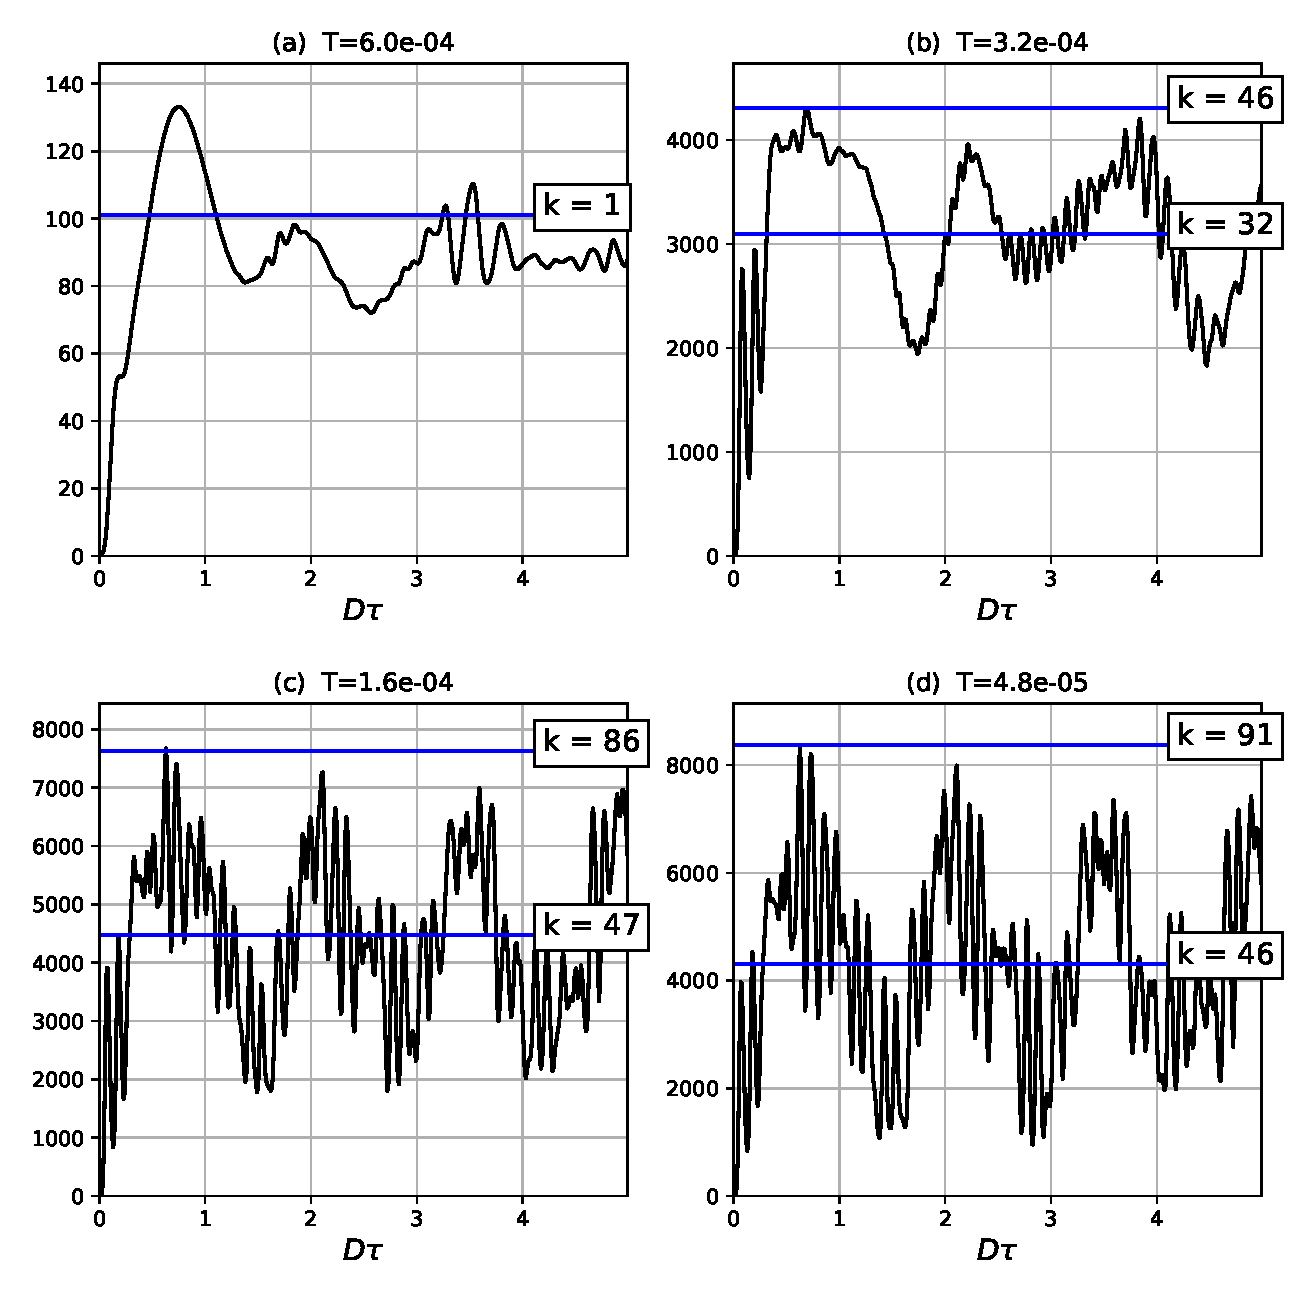
\includegraphics[width=0.95\linewidth]{fisher_low_bound_n101.eps}
	\caption{
	  Зависимость нижней границы  квантовой информации Фишера $F_\mathrm{Q} = 2 M_{2}$
	  от безразмерного времени $D\tau$ при $N=101$.
	  a) $T=6\cdot10^{-4}$~K, неравенство~(\ref{eq:20}) определяет область парной запутанности  (k+1=2), эта область выше горизонтальной линии;
	  b) $T=3.2\cdot10^{-4}$~K, область многоспиновой запутанности представляет собой полосу, ограниченную горизонтальными линиями с~$k=19$~и~$k=46$;
	  c) $T = 1.6\cdot10^{_4}$~K, горизонтальные линии ($k=18$ и $k=86$) ограничивают полосу с многоспиновой запутанностью;
	  d) при $T=4.8\cdot10^{-5}$~K возникают запутанные кластеры с $11-92$ спинами.
	}
	\label{fig:2}
\end{figure}

Рассматриваемая модель спин-несущих молекул (атомов) в нанопоре в дипольном упорядоченном состоянии расширяет возможности исследования многоспиновой запутанности по сравнению с родственной моделью~\cite{Doronin_2019},
в которой система изначально находилась в термодинамическом равновесии в сильном внешнем магнитном поле.
Модель~\cite{Doronin_2019} неприменима для исследования эволюции системы во времени,
потому что распределение МК~когерентностей~ЯМР~быстро становится стационарным~\cite{Doronin_2009}.
Многоспиновая запутанность изменяется с температурой в очень узком температурном интервале в модели~\cite{Doronin_2019}.
Например, все спины запутаны в системе, состоящей из 201 спина уже при температуре $T=6.856\cdot10^{-3}$~K~\cite{Doronin_2019}.

 Зависимость квантовой информации Фишера от времени в системе, состоящей из 101 спина, представлена на Рис.~(\ref{fig:2}) при различных температурах.
Из Рис.~(\ref{fig:2}a) видно, что при температуре $T=6\cdot10^{-4}$~K существует только парная запутанность.
При температуре $T=3.2\cdot10^{-4}$ на Рис.~(\ref{fig:2}b) появляется полоса, в которой неравенство~(\ref{eq:20}) может быть выполнено, когда $19 \leq k \leq 46$.
Таким образом, существует многоспиновая запутанность в спиновых кластерах, состоящих из 20-47 спинов, при температуре $3.2\cdot10^{-4}$~K.
Когда температура понижается, ширина полосы, в которой существует многоспиновая запутанность, увеличивается.
При температуре $T=1.6\cdot10^{-4}$~K (Рис.~(\ref{fig:2}c)) появляются кластеры из 19-87 запутанных спинов, а при температуре $T=4.8\cdot10^{-5}$~K (Рис.~(\ref{fig:2}d)), наблюдаются 11-92 запутанных спина.

\begin{figure}
 	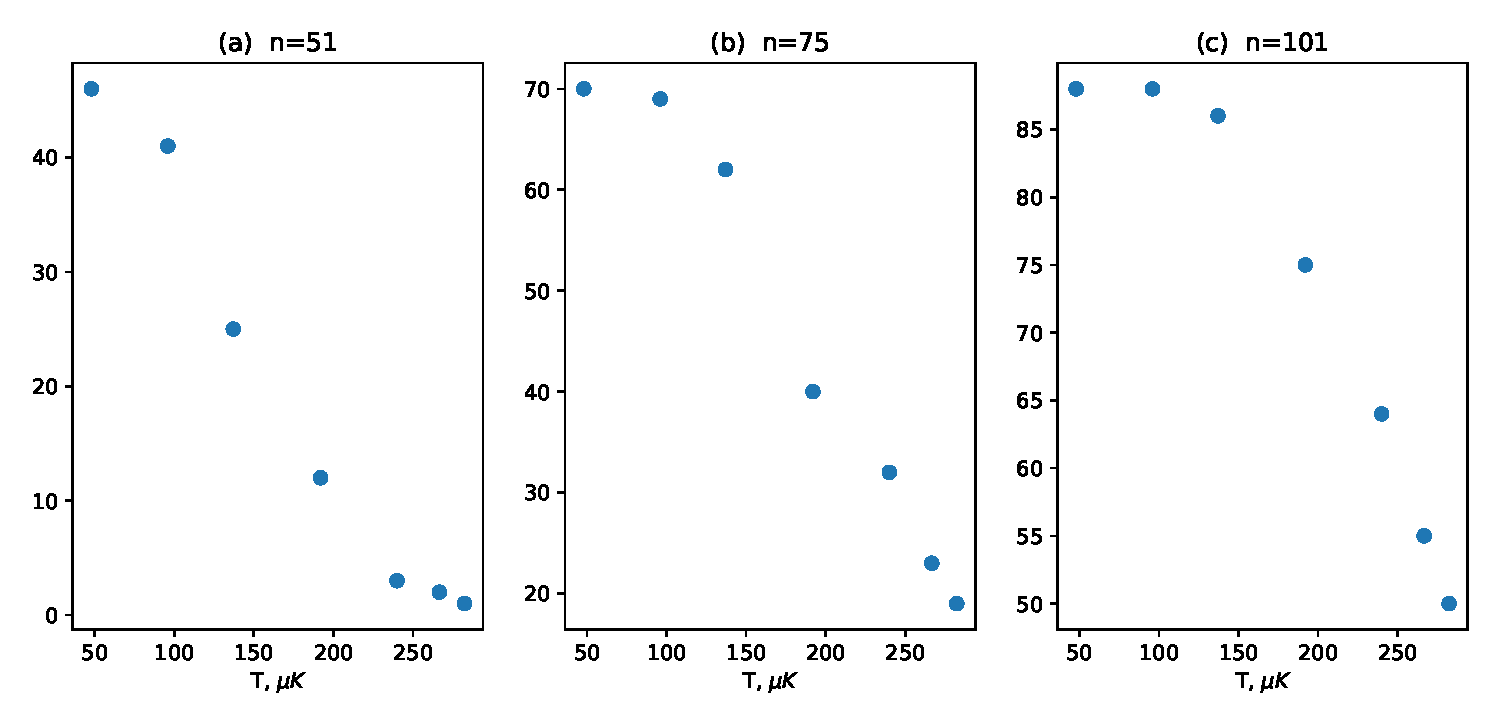
\includegraphics[width=0.95\linewidth]{entangled_spins_by_n.eps}
	\caption{
	  Зависимость максимального количества запутанных спинов,
	  усредненного по времени эволюции $(0 \leq D\tau \leq 3)$,
	  от температуры при  a) $N=51$; b) $N=75$; c) $N=101$.
	}
	\label{fig:3}
\end{figure}

Зависимость максимального числа запутанных спинов за время эволюции $({0}\leq \mathrm{D}\tau\leq{3})$ от температуры при разных числах спинов в нанопоре представлена на Рис.~(\ref{fig:3}).
Максимальное количество запутанных спинов уменьшается при повышении температуры.
Максимальное количество запутанных спинов увеличивается, когда увеличивается число спинов в нанопоре, потому что система в нанопоре становится плотнее.



\section{Заключение}
\label{sec:6}

Мы исследовали многоспиновую запутанность в системе спин-несущих молекул (атомов), заполняющих несферические нанопоры в условиях эксперимента МК~спектроскопии~ЯМР~.
Спины изначально находились в дипольном упорядоченном состоянии.
Найдена зависимость многоспиновой запутанности от температуры и количества спинов в нанопоре.

Проведенные исследования позволяют заключить, что МК~спектроскопия~ЯМР~является тонким и полезным методом для исследования различных проблем квантовой информатики.
В частности, это очень эффективный метод исследования квантовой запутанности.


\section{Благодарности}
Эта работа выполнена в рамках Государственного задания, госрегистрация № 0089-2019-0002.
Работа частично поддержана Российским фондом фундаментальных исследований (гранты № 20-03-00147, 19-32-80004).
И.Л. благодарит Фонд развития теоретической физики «БАЗИС» №19-1-5-130-1.



\appendix
\section{Двухимпульсный эксперимент Брокаерта-Джинера при низкой зеемановской температуре и высокой дипольной температуре.}

Изначально система находится в состоянии термодинамического равновесия в сильном внешнем магнитном поле с матрицей плотности
%
\begin{equation}
  \label{eq:a1}
  \sigma_{i} = \dfrac{e^{\beta_\mathrm{L} \omega_{0} I_\mathrm{z}}}{Z_{i}} ,
  \quad
  Z_{i} = \mathrm{Tr}\left\{e^{\beta_\mathrm{L} \omega_{0} I_\mathrm{z}} \right\}
\end{equation}
%
После первого резонансного $x$-импульса получаем
%
\begin{equation}
  \label{eq:a2}
  \sigma'(0) = e^{ i \frac \pi 2 I_\mathrm{x}}
  \sigma_{i}
  e^{-i \frac \pi 2 I_\mathrm{x}}
  = \dfrac{e^{\beta_\mathrm{L} \omega_{0} I_\mathrm{y}}}{Z_{i}} .
\end{equation}
%
Затем система свободно эволюционирует в течение времени $\tau$,
и после этого подается второй резонансный $y$-импульс, который поворачивает спины на угол $\theta$ вокруг оси-$y$ ВСК.
В результате получаем, что
\begin{equation}
  \label{eq:a3}
  \sigma'(\tau)
  = \dfrac{
   e^{-i \theta I_\mathrm{y}} e^{-i H_\mathrm{dz} \tau}
   e^{\beta_\mathrm{L} \omega_{0} I_\mathrm{y}}
   e^{i H_\mathrm{dz} \tau} e^{i \theta I_\mathrm{y}}
  }{Z_{i}}.
\end{equation}
%
По истечении времени $T_2$ ($T_2$ - время спиновой релаксации \cite{Goldman_1970}) система достигает состояния термодинамического равновесия
\begin{equation}
  \label{eq:a4}
  \sigma_{f}
  = \dfrac{ e^{\alpha \omega_{0} I_\mathrm{z} + \beta H_\mathrm{dz}} }{Z_f},
\end{equation}
%
где $\alpha$ и $\beta$ - обратные зеемановская и дипольная температуры.
Очевидно, что система имеет единственное  равновесное состояние, а
 температуры $\alpha$ и $\beta$ в равновесном состоянии находятся из
законов сохранения:

\begin{align}
  \label{eq:a5}
  \mathrm{Tr} \left\{ I_\mathrm{z} \sigma'(\tau) \right\}
  & = \mathrm{Tr} \left\{ I_\mathrm{z} \sigma_{f}(\tau) \right\}
  \\
  \label{eq:a6}
  \mathrm{Tr} \left\{ H_\mathrm{dz} \sigma'(\tau) \right\}
  & = \mathrm{Tr} \left\{ H_\mathrm{dz} \sigma_{f}(\tau) \right\}
\end{align}
%
Можно переписать $\mathrm{Tr} \left\{ I_\mathrm{z} \sigma'(\tau) \right\}$ как
%
\begin{multline}
  \label{eq:a7}
  \tr{I_\mathrm{z} \sigma'(\tau)}
  = \dfrac{1}{Z_{i}} \tr{
    e^{i \theta \sy} \sz e^{-i \theta \sy}
    e^{-i \hdz \tau} e^{\beta_\mathrm{L} \omega_{0} \sy} e^{i \hdz \tau}
  }
  \\
  = \dfrac{1}{Z_i} \tr{
    \left( \cos(\theta) \sz - \sin(\theta) \sx \right)
    e^{-i \hdz \tau} e^{\beta_\mathrm{L} \omega_{0} \sy} e^{i \hdz \tau}
  }
  \\
  = \dfrac{1}{Z_i} \tr{
    e^{-i \pi \sy}
    \left( \cos(\theta) \sz - \sin(\theta) \sx \right)
    e^{-i \hdz \tau} e^{\beta_\mathrm{L} \omega_{0} \sy} e^{i \hdz \tau}
    e^{i \pi \sy}
  }
  \\
  = - \dfrac{1}{Z_i} \tr{
    \left( \cos(\theta) \sz - \sin(\theta) \sx \right)
    e^{-i \hdz \tau} e^{\beta_\mathrm{L} \omega_{0} \sy} e^{i \hdz \tau}
  } = 0
\end{multline}
%
В~(\ref{eq:a7}) было учтено, что $\left[ e^{-i \pi \sy}, \hdz \right] = 0$.
Поскольку мы рассматриваем случай высокой дипольной температуры, можно переписать уравнение~(\ref{eq:a5}) как
\begin{equation}
  \label{eq:a8}
  0 = \dfrac{1}{Z_f} \tr{ \sz e^{\alpha \omega_0 \sz}}
  + \dfrac{\beta}{Z_f} \tr{\sz e^{\alpha \omega_0 \sz} \hdz}.
\end{equation}
%
Заметим, что $\tr{\sz} = \tr{\sz\hdz} = 0$.
В таком случае $\alpha = 0$ удовлетворяет уравнению~(\ref{eq:5}).
Таким образом, в рассматриваемом случае мы получаем дипольном упорядоченное состояние.

%%%%%%%%%%%%%%%%%%%%%%%%%%%%%
\bibliography{bibliography}
\end{document}
